\part{Lecture 11: Stochastic Policy Gradient Methods}
\title[RL Lecture 11]{Lecture 11: Stochastic Policy Gradient Methods}  
\date{}  
\frame{\titlepage} 

%%%%%%%%%%%%%%%%%%%%%%%%%%%%%%%%%%%%%%%%%%%%%%%%%%%%%%%%%%%%%
%% Preface (1) %%
%%%%%%%%%%%%%%%%%%%%%%%%%%%%%%%%%%%%%%%%%%%%%%%%%%%%%%%%%%%%%
\frame{\frametitle{Preface (1)}
Shift from (indirect) value-based approaches
\begin{equation}
			\hat{q}(\bm{x}, u, \bm{w}) \approx q(\bm{x}, u)
\end{equation}
to (direct) policy-based solutions:
\begin{equation}
	\bm{\pi}(\bm{u}|\bm{x})=\Pb{\bm{U} = \bm{u} | \bm{X} = \bm{x}}\approx\bm{\pi}(\bm{u}|\bm{x}, \bm{\theta})\, .
\end{equation}\pause
\begin{itemize}
	\item Above, $\bm{\theta}\in \mathbb{R}^d$ is the policy parameter vector.
	\item Note, that $\bm{u}$ is now vectorial and might contain multiple continuous quantities. 
\end{itemize}
\pause
\begin{block}{Goal of today's lecture}
\begin{itemize}
	\item Introduce an algorithm class based on a parameterizable policy $\pi(\bm{\theta})$.
	\item Extend the action space to continuous actions.
	\item Combine the policy-based and value-based approach.
\end{itemize}
\end{block}
}

%%%%%%%%%%%%%%%%%%%%%%%%%%%%%%%%%%%%%%%%%%%%%%%%%%%%%%%%%%%%%
%% Preface (2) %%
%%%%%%%%%%%%%%%%%%%%%%%%%%%%%%%%%%%%%%%%%%%%%%%%%%%%%%%%%%%%%
\frame{\frametitle{Preface (2)}
\begin{figure}
	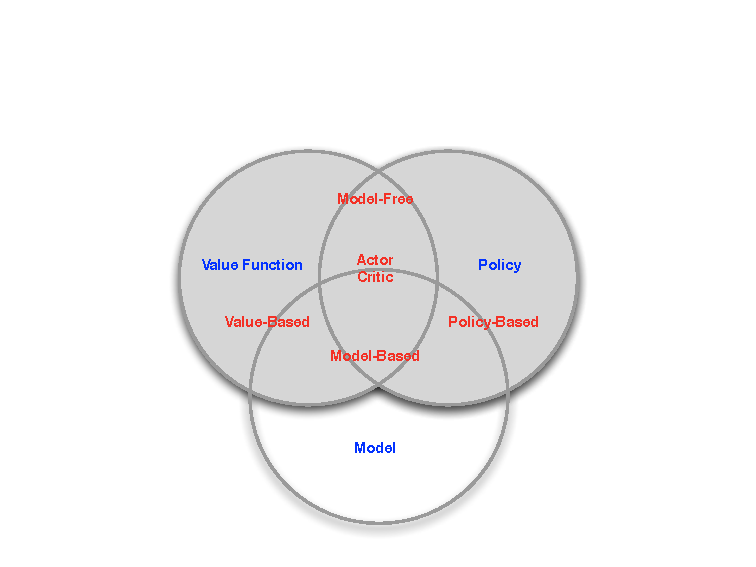
\includegraphics[height=0.7\textheight]{fig/lec01/RL_Agent_Taxonomy.pdf}
	\caption{Main categories of reinforcement learning algorithms\\  \SilverLectureSource}
\end{figure}
}

%%%%%%%%%%%%%%%%%%%%%%%%%%%%%%%%%%%%%%%%%%%%%%%%%%%%%%%%%%%%%%%%%%
\section{Stochastic policy approximation and the policy gradient theorem} 
%%%%%%%%%%%%%%%%%%%%%%%%%%%%%%%%%%%%%%%%%%%%%%%%%%%%%%%%%%%%%%%%%%
\begin{frame}
\frametitle{Table of contents}
\tableofcontents
\end{frame}


%%%%%%%%%%%%%%%%%%%%%%%%%%%%%%%%%%%%%%%%%%%%%%%%%%%%%%%%%%%%%
%% Motivating Example (2): Strategic Gaming %%
%%%%%%%%%%%%%%%%%%%%%%%%%%%%%%%%%%%%%%%%%%%%%%%%%%%%%%%%%%%%%
\frame{\frametitle{Motivating example: strategic gaming}
\onslide<1->Task: Two-player game of extended rock-paper-scissors 
\begin{itemize}
	\onslide<2->\item A deterministic policy (i.e., value-based with given feature representation) can be easily exploited by the opponent.
	\onslide<3->\item	Conversely, a uniform random policy would be unpredictable.
\end{itemize}

\onslide<1->
\begin{figure}
	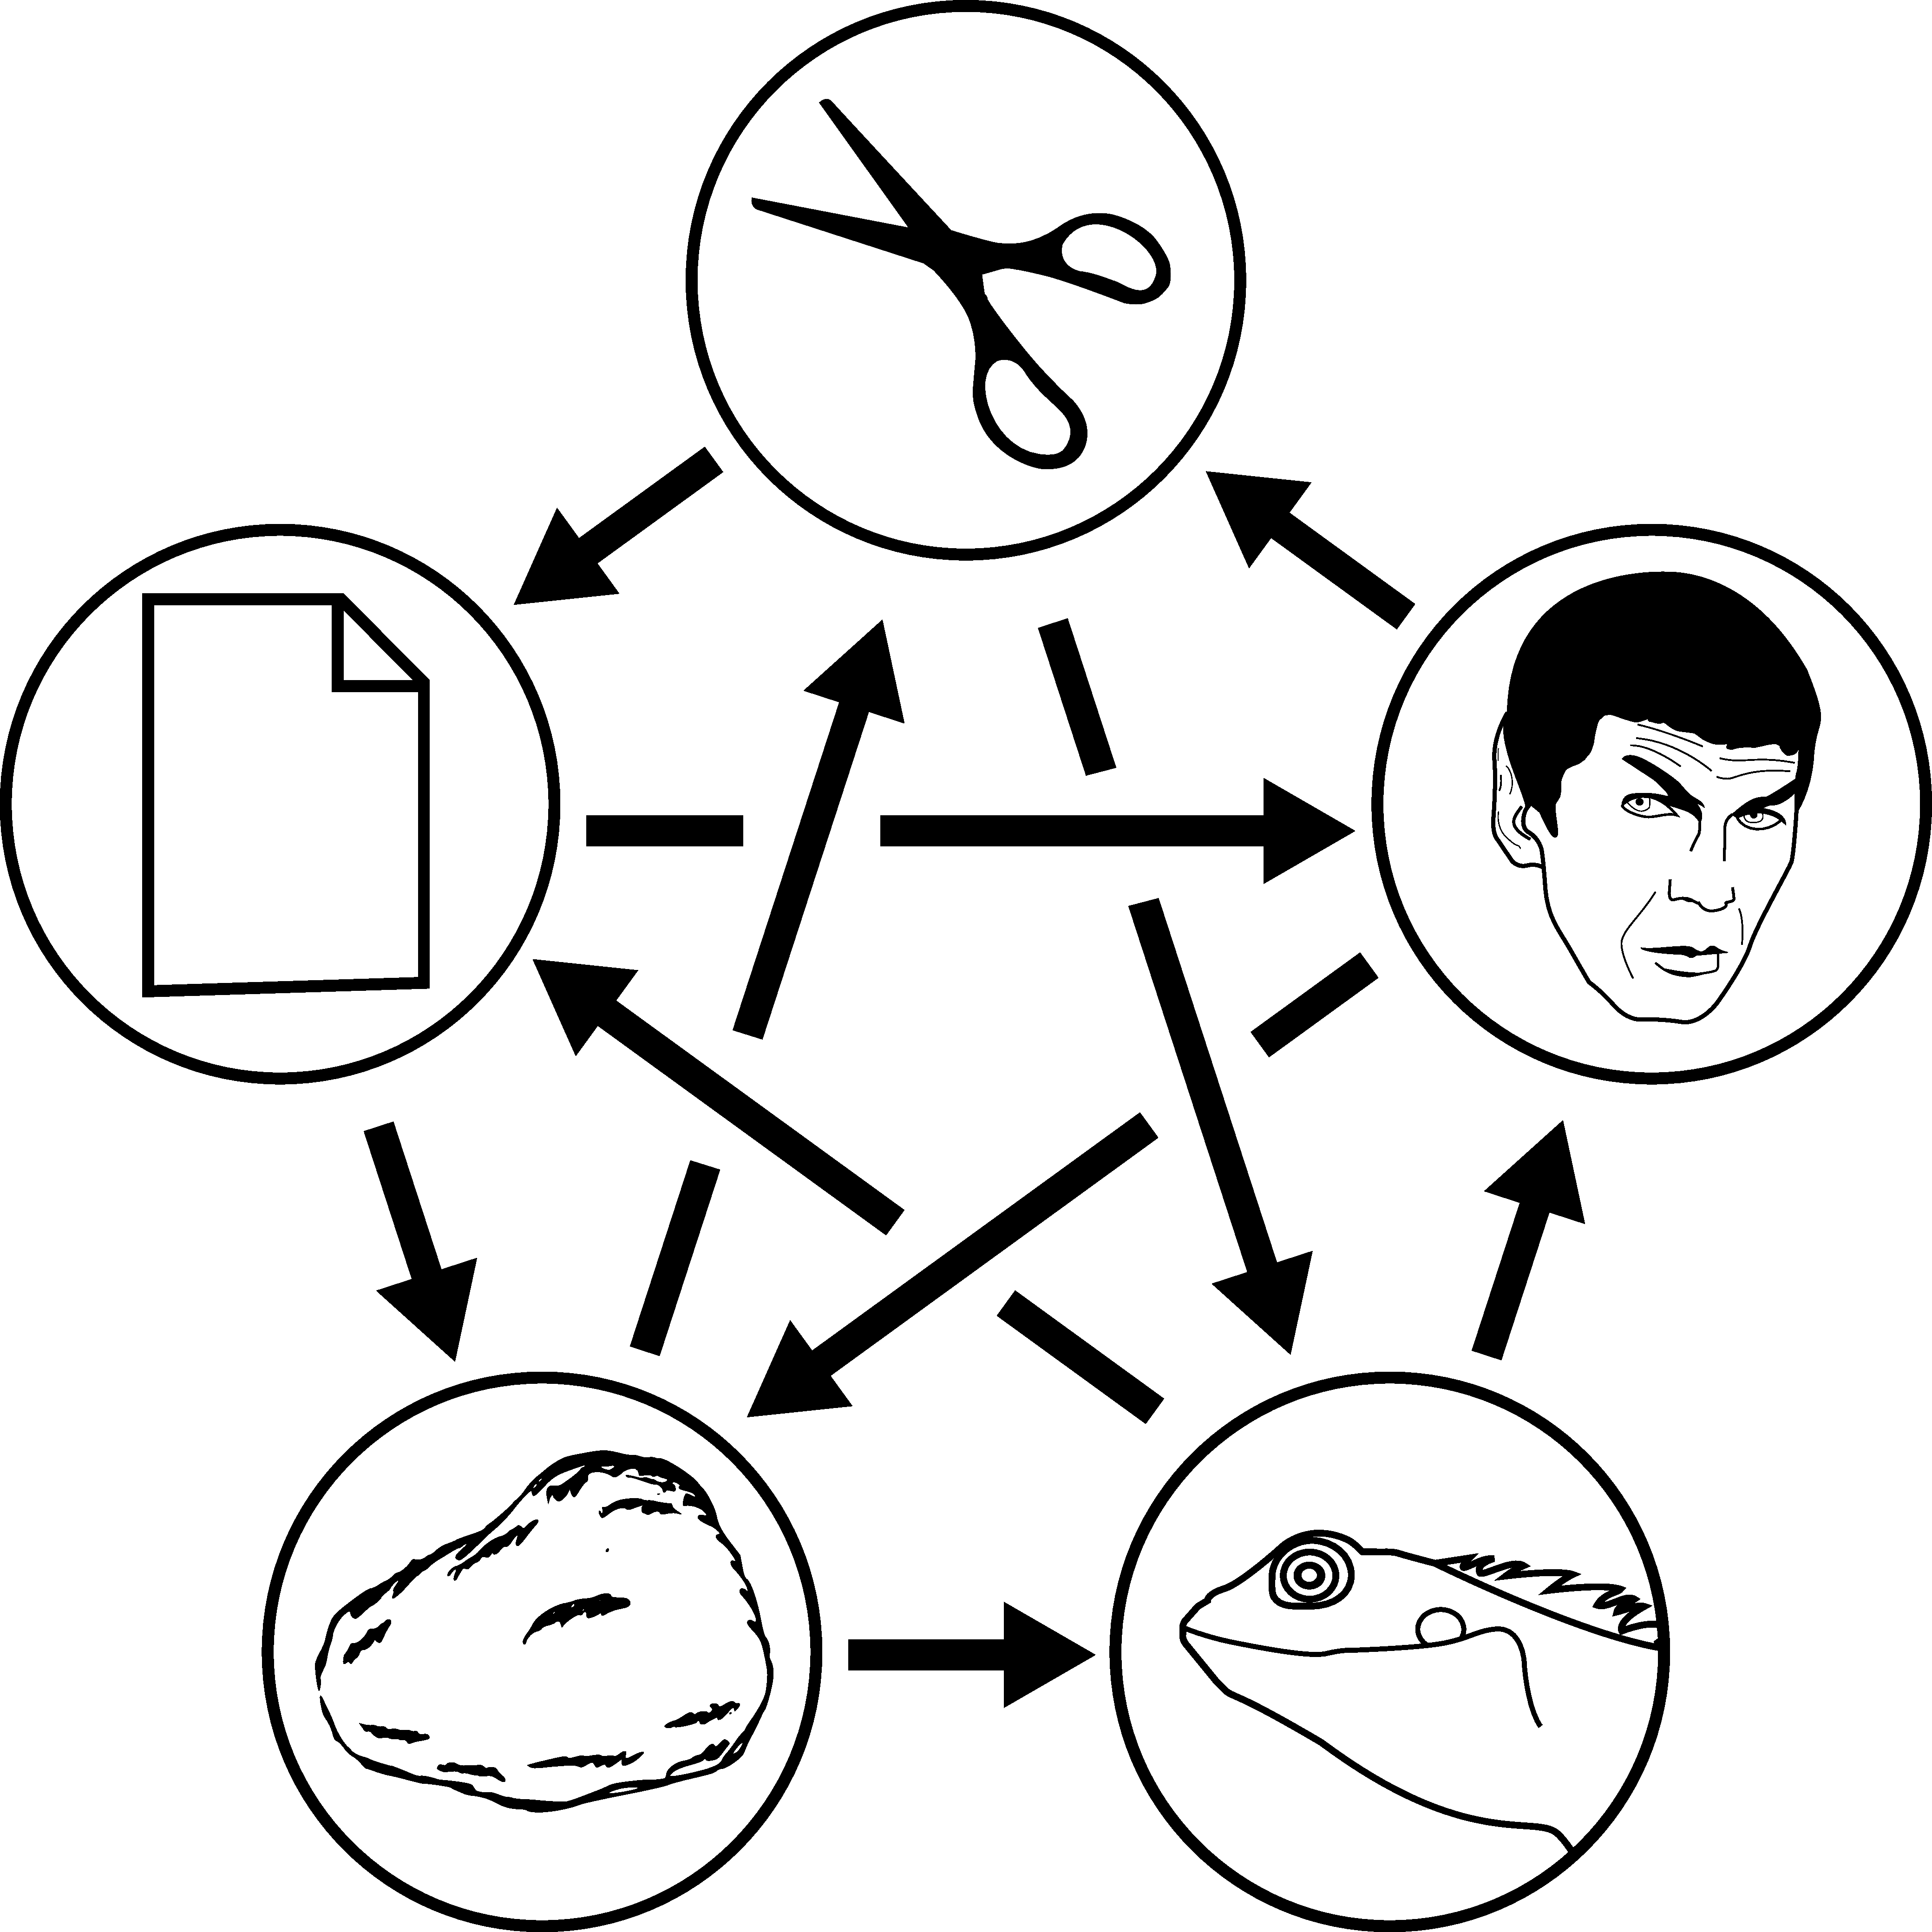
\includegraphics[height=0.5\textheight]{fig/lec01/Rock_paper_scissors_lizard_spock.pdf}
	\caption{Rock paper scissors lizard Spock game mechanics\\(source: \href{https://commons.wikimedia.org/wiki/File:Rock_paper_scissors_lizard_spock.svg}{www.wikipedia.org},  by \href{https://en.wikipedia.org/wiki/User:Diriector_Doc}{Diriector Doc} \href{https://creativecommons.org/licenses/by-sa/4.0/deed.en}{CC BY-SA 4.0})}
\end{figure}
}

%%%%%%%%%%%%%%%%%%%%%%%%%%%%%%%%%%%%%%%%%%%%%%%%%%%%%%%%%%%%%
%% Example Policy Function: Discrete Action Space %%
%%%%%%%%%%%%%%%%%%%%%%%%%%%%%%%%%%%%%%%%%%%%%%%%%%%%%%%%%%%%%
\frame{\frametitle{Example policy function: discrete action space}
Assumption:
\begin{itemize}
	\item Action space is discrete and compact.
\end{itemize}\pause
A typical policy function is:
\begin{itemize}
	\item \hl{Soft-max in action preferences}
	\begin{equation}
		\pi(u|\bm{x},\bm{\theta}) = \frac{e^{h(\bm{x},u,\bm{\theta})}}{\sum_i e^{h(\bm{x},i,\bm{\theta})}}
		\label{eq:soft_max_preference}
	\end{equation}
	with $h(\bm{x},u,\bm{\theta}):\mathcal{X}\times\mathcal{U}\times\mathbb{R}^d \rightarrow \mathbb{R}$ being the numerical preference per state-action pair.\pause
	\item Denominator of \eqref{eq:soft_max_preference} sums up action probabilities to one per state. \pause
	\item Is designed as a stochastic policy but can approach deterministic behavior in the limit. \pause
	\item The preference is parametrized via a function approximator, e.g., linear in features
	\begin{equation}
		h(\bm{x},u,\bm{\theta}) = \bm{\theta}\T\tilde{\bm{x}}(\bm{x}, u).
	\end{equation}
\end{itemize}
}

%%%%%%%%%%%%%%%%%%%%%%%%%%%%%%%%%%%%%%%%%%%%%%%%%%%%%%%%%%%%%
%% Example Policy Function: Continuous Action Space (1) %%
%%%%%%%%%%%%%%%%%%%%%%%%%%%%%%%%%%%%%%%%%%%%%%%%%%%%%%%%%%%%%
\frame{\frametitle{Example policy function: continuous action space (1)}
Assumption:
\begin{itemize}
	\item Action space is continuous and there is only one scalar action $u\in\mathbb{R}$.
\end{itemize}\pause
A typical policy function is:
\begin{itemize}
	\item \hl{Gaussian probability density}
	\begin{equation}
		\pi(u|\bm{x},\bm{\theta}) = \frac{1}{\sigma(\bm{x},\bm{\theta})\sqrt{2\pi}}\exp\left(-\frac{(u-\mu(\bm{x},\bm{\theta}))^2}{2\sigma(\bm{x},\bm{\theta})^2}\right)
		\label{eq:gaussian_action}
	\end{equation}
	with mean $\mu(\bm{x},\bm{\theta}):\mathcal{X}\times\mathbb{R}^d \rightarrow \mathbb{R}$ and standard deviation $\sigma(\bm{x},\bm{\theta}):\mathcal{X}\times\mathbb{R}^d \rightarrow \mathbb{R}$ given by parametric function approximation.\pause
		\item Variants regarding function $\mu$ and $\sigma$:
	\begin{enumerate}
		\item Both  share a mutual parameter set $\bm{\theta}$ (e.g., artificial neural network with multiple outputs).\pause
		\item Both are parametrized independently $\bm{\theta}=\begin{bmatrix}\bm{\theta}_\mu & \bm{\theta}_\sigma\end{bmatrix}\T$ (e.g., by two linear regression functions).\pause
		\item Only $\mu(\bm{x},\bm{\theta})$ is parametrized while $\sigma$ is scheduled externally. 
	\end{enumerate}
\end{itemize}
}

%%%%%%%%%%%%%%%%%%%%%%%%%%%%%%%%%%%%%%%%%%%%%%%%%%%%%%%%%%%%%
%% Example Policy Function: Continuous Action Space (2) %%
%%%%%%%%%%%%%%%%%%%%%%%%%%%%%%%%%%%%%%%%%%%%%%%%%%%%%%%%%%%%%
\frame{\frametitle{Example policy function: continuous action space (2)}
\begin{itemize}
	\item Output of the functions $\mu_k=(\bm{x}_k,\bm{\theta}_k)$ and $\sigma_k=(\bm{x}_k,\bm{\theta}_k)$ can change in every time step.
	\item Depending on $\sigma$ exploration is an inherent part of the (stochastic) policy. 
\end{itemize}
\begin{figure}
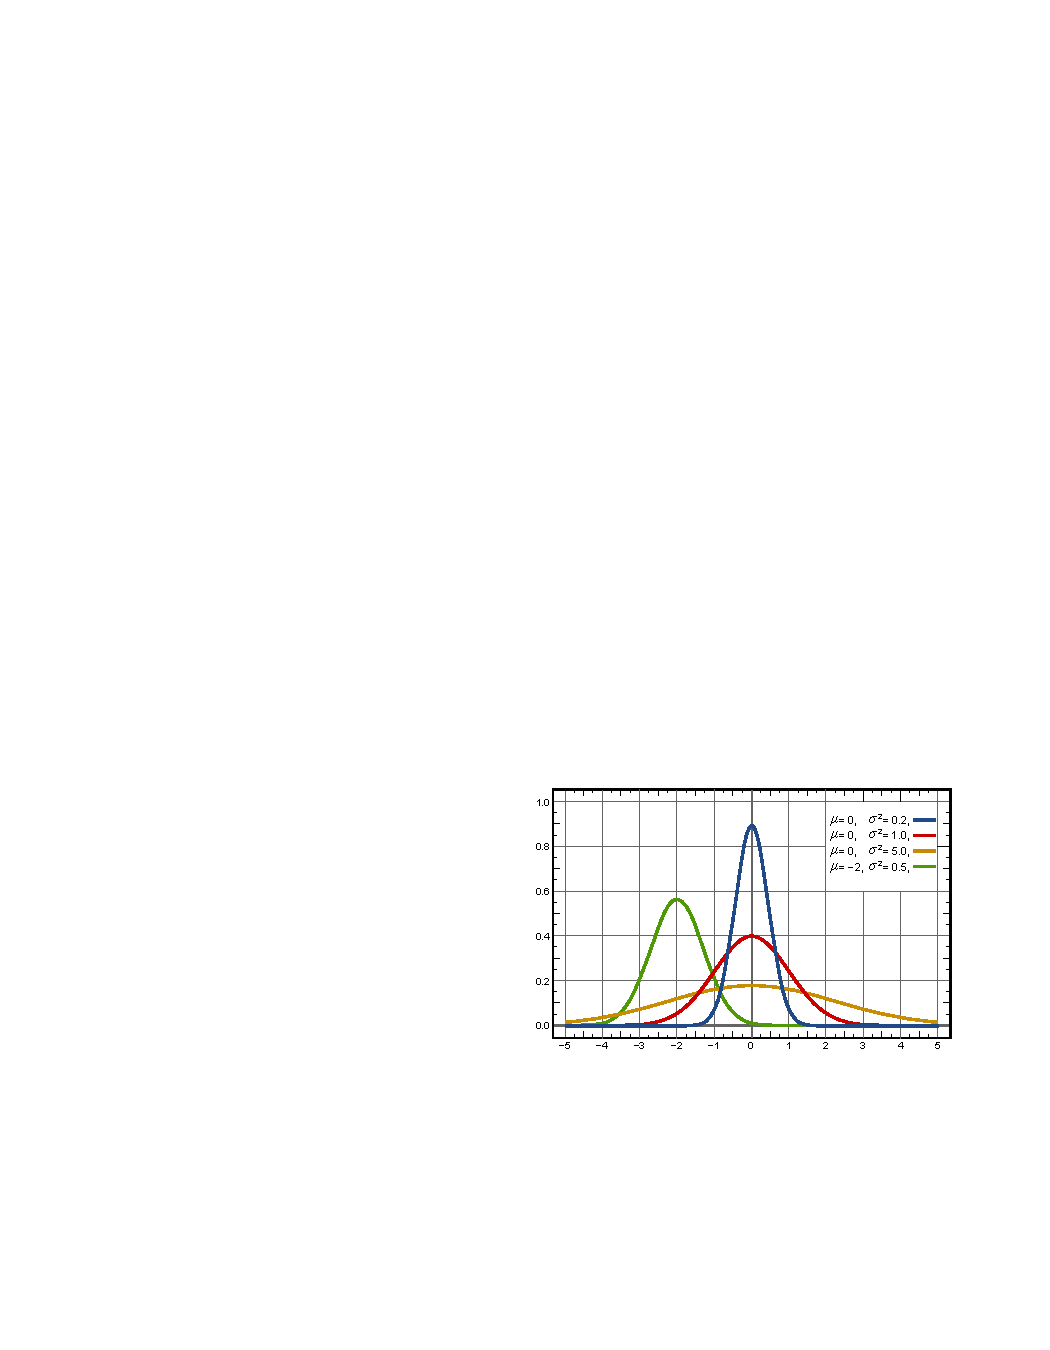
\includegraphics[width=5.5cm]{fig/lec11/Gaussian_Distri.pdf}
\caption{Exemplary univariate Gaussian probability density functions (source: R. Sutton and G. Barto, Reinforcement learning: an introduction, 2018, \href{https://creativecommons.org/licenses/by-nc-nd/2.0/}{CC BY-NC-ND 2.0})}
\label{fig:Gaussian_Distri}
\end{figure}
}

%%%%%%%%%%%%%%%%%%%%%%%%%%%%%%%%%%%%%%%%%%%%%%%%%%%%%%%%%%%%%
%% Example Policy Function: Continuous Action Space (3) %%
%%%%%%%%%%%%%%%%%%%%%%%%%%%%%%%%%%%%%%%%%%%%%%%%%%%%%%%%%%%%%
\frame{\frametitle{Example policy function: continuous action space (3)}
Assumption:
\begin{itemize}
	\item Action space is continuous and there are multiple actions $\bm{u}\in\mathbb{R}^m$.
\end{itemize} \pause
A typical policy function is:
\begin{itemize}
	\item \hl{Multivariate Gaussian probability density}
	\begin{equation}
		\pi(\bm{u}|\bm{x},\bm{\theta}) = \frac{1}{\sqrt{(2\pi)^m\det(\bm{\Sigma})}}\exp\left(-\frac{1}{2}(\bm{u}-\bm{\mu})\T\bm{\Sigma}^{-1}(\bm{u}-\bm{\mu})\right)
		\label{eq:gaussian_action_multivariate}
	\end{equation}
	with mean $\bm{\mu}(\bm{x},\bm{\theta}):\mathcal{X}\times\mathbb{R}^d \rightarrow \mathbb{R}^m$ and covariance matrix $\bm{\Sigma}(\bm{x},\bm{\theta}):\mathcal{X}\times\mathbb{R}^d \rightarrow \mathbb{R}^{m \times m }$ given by parametric function approximation. \pause
		\item Same parametrization variants apply to $\bm{\mu}$ and $\bm{\Sigma}$ as in the scalar action case. \pause
		\item In addition, $\bm{\Sigma}$ can be considered a diagonal matrix and clipped to reduce complexity as well as ensure nonsingularity.
\end{itemize}
}

%%%%%%%%%%%%%%%%%%%%%%%%%%%%%%%%%%%%%%%%%%%%%%%%%%%%%%%%%%%%%
%% Example Policy Function: Continuous Action Space (4) %%
%%%%%%%%%%%%%%%%%%%%%%%%%%%%%%%%%%%%%%%%%%%%%%%%%%%%%%%%%%%%%
\frame{\frametitle{Example policy function: continuous action space (4)}
\begin{itemize}
	\item Below we find an example for 
\end{itemize}
\begin{equation*}
	\bm{\mu}=\begin{bmatrix}-0.4 & 0.3\end{bmatrix}\T \quad \mbox{and} \quad \bm{\Sigma}=\begin{bmatrix}0.04 & 0\\ 0 & 0.02 \end{bmatrix} .
\end{equation*}
\begin{figure}
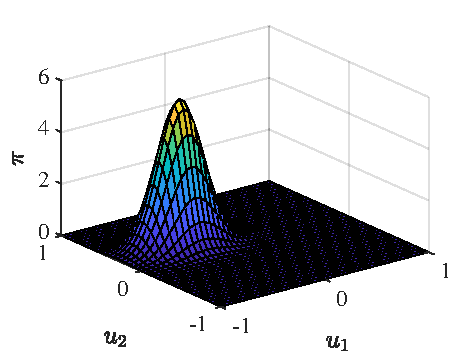
\includegraphics[width=6.5cm]{fig/lec11/Gaussian_Policy_Multivariate.pdf}
\caption{Exemplary bivariate Gaussian probability density function}
\label{fig:Gaussian_Policy_Multivariate}
\end{figure}
}

%%%%%%%%%%%%%%%%%%%%%%%%%%%%%%%%%%%%%%%%%%%%%%%%%%%%%%%%%%%%%
%% Policy Objective Function %%
%%%%%%%%%%%%%%%%%%%%%%%%%%%%%%%%%%%%%%%%%%%%%%%%%%%%%%%%%%%%%
\frame{\frametitle{Policy objective function}
\begin{itemize}
	\item Goal: find optimal $\bm{\theta}^*$ given the policy $\bm{\pi}(\bm{u}|\bm{x}, \bm{\theta})$. \pause
	\item Problem: which measure of optimality should we use? \pause
\end{itemize}
\vspace{0.5cm}
Possible optimality metrics:
\begin{itemize}
	\item \hl{Start state value} (in episodic tasks):
	\begin{equation}
		J(\bm{\theta}) = v_{\pi_{\bm{\theta}}}(\bm{x}_0)=\E{v|\bm{X}=\bm{x}_0, \bm{\theta}}
		\label{eq:performance_metric_episodic}
	\end{equation}\pause
	\item \hl{Average reward} (in continuing tasks):
	\begin{equation}
		J(\bm{\theta}) = \overline{r}_{\pi_{\bm{\theta}}} = \int_\mathcal{X}\mu_\pi(\bm{x})\int_\mathcal{U}\pi(\bm{u}|\bm{x}, \bm{\theta})\int_{\mathcal{X},\mathcal{R}}p(\bm{x}', r|\bm{x},\bm{u})r
		\label{eq:performance_metric_continuing}
	\end{equation}
	\begin{itemize}
		\item Above, $\mu_\pi(\bm{x})$ is again the steady-state distribution $\mu_\pi(\bm{x})=\lim_{k\rightarrow\infty}\Pb{\bm{X}_k=\bm{x}|\bm{U}_{0:k-1}\sim\pi}$.
	\end{itemize}
\end{itemize}
}

%%%%%%%%%%%%%%%%%%%%%%%%%%%%%%%%%%%%%%%%%%%%%%%%%%%%%%%%%%%%%
%% Policy Optimization %%
%%%%%%%%%%%%%%%%%%%%%%%%%%%%%%%%%%%%%%%%%%%%%%%%%%%%%%%%%%%%%
\frame{\frametitle{Policy optimization}
\begin{itemize}
	\onslide<1->\item In essence, policy-based RL is an \hl{optimization problem}.
	\onslide<2->{\item Depending on the policy function and task, finding $\bm{\theta}^*$ might be a 
	\begin{itemize}
		\item non-linear,
		\item multidimensional and
		\item non-stationary problem.
	\end{itemize}}
	\onslide<3->{\item Hence, we might consider global optimization techniques\footnote[1]{\onslide<3->{Recommended reading: J. Stork et al., \textit{A new Taxonomy of Continuous Global Optimization Algorithms}, \href{https://arxiv.org/abs/1808.08818}{https://arxiv.org/abs/1808.08818}, 2020}} like
		\begin{itemize}
		\item Simple heuristics: random search, grid search,...}
		\onslide<4->\item Meta-heuristics: evolutionary algorithms, particle swarm,.... 
		\onslide<5->\item Surrogate-model-based optimization: Bayes opt.,...
		\onslide<6->\item Gradient-based techniques with multi-start initialization.
	\end{itemize}
\end{itemize}
}

%%%%%%%%%%%%%%%%%%%%%%%%%%%%%%%%%%%%%%%%%%%%%%%%%%%%%%%%%%%%%
%% How to Retrieve the Gradient? %%
%%%%%%%%%%%%%%%%%%%%%%%%%%%%%%%%%%%%%%%%%%%%%%%%%%%%%%%%%%%%%
\frame{\frametitle{Policy gradient}
\begin{columns}[t,onlytextwidth]
\begin{column}{0.475\textwidth}
\begin{minipage}[c]{\linewidth}
\begin{figure}
	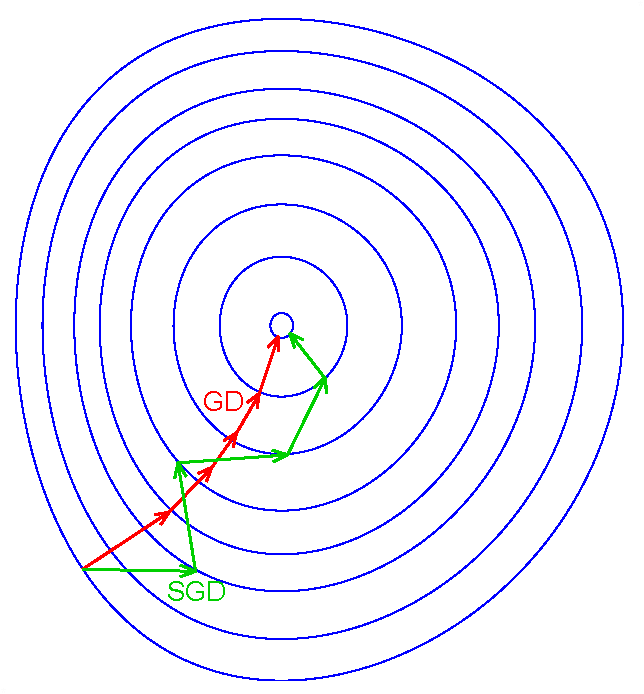
\includegraphics[width=4.5cm]{fig/lec11/Gradient_ascent.pdf}
	\caption{Exemplary optimization paths for (stochastic) gradient ascent \\(derivative work of \href{https://commons.wikimedia.org/wiki/File:Gradient_descent.svg}{www.wikipedia.org}, \href{https://creativecommons.org/publicdomain/zero/1.0/deed.en}{CC0 1.0})}
	\label{fig:Gradient_ascent}
\end{figure}
\end{minipage}
\end{column}
\hfill
\begin{column}{0.54\textwidth}
\begin{minipage}[c]{\linewidth}
\begin{itemize}
	\item We will focus on gradient-based methods (\hl{policy gradient}).\pause
	\item Hence, we will assume that the gradient
	\begin{equation*}
		\nabla_{\bm{\theta}} J(\bm{\theta})=\begin{bmatrix}\frac{\partial J}{\partial \theta_1} & \cdots & \frac{\partial J}{\partial \theta_d} \end{bmatrix}\T
	\end{equation*}
	required for \hl{gradient ascent optimization} always exists:
	\begin{equation*}
		\bm{\theta} \leftarrow\bm{\theta} + \alpha \nabla_{\bm{\theta}} J(\bm{\theta}).
	\end{equation*}\pause\vspace{-0.4cm}
	\item True gradient $\nabla_{\bm{\theta}} J(\bm{\theta})$ is usually approximated, e.g., by stochastic gradient descent (SGD) or derived variants.
\end{itemize}
\end{minipage}
\end{column}
\end{columns}
}

%%%%%%%%%%%%%%%%%%%%%%%%%%%%%%%%%%%%%%%%%%%%%%%%%%%%%%%%%%%%%
%% Policy Gradient Theorem %%
%%%%%%%%%%%%%%%%%%%%%%%%%%%%%%%%%%%%%%%%%%%%%%%%%%%%%%%%%%%%%
\frame{\frametitle{Policy gradient theorem}
\begin{theo}{Policy Gradient}{policy_gradient}
Given a metric $J(\bm{\theta})$ for the undiscounted episodic \eqref{eq:performance_metric_episodic} or continuing tasks \eqref{eq:performance_metric_continuing} and a parameterizable policy $\pi(\bm{u}|\bm{x},\bm{\theta})$ the policy gradient is
\begin{equation}
	\nabla_{\bm{\theta}} J(\bm{\theta}) = \El{q_{\pi}(\bm{x},\bm{u})\frac{\nabla_{\bm{\theta}}\pi(\bm{u}|\bm{x},\bm{\theta})}{\pi(\bm{u}|\bm{x},\bm{\theta})}}{\pi}.
	\label{eq:policy_gradient_theo}
\end{equation}
\end{theo}\pause
\begin{itemize}
 \item Having samples $\left\langle\bm{x}_i, \bm{u}_i \right\rangle$, an estimate of $q_{\pi}$ and the policy function $\pi(\bm{\theta})$ available we receive an \hl{analytical solution for the policy gradient!} \pause
\item Using identity $\nabla \ln a = \frac{\nabla a}{a}$ we can re-write to
\begin{equation}
	\nabla_{\bm{\theta}} J(\bm{\theta}) = \El{q_{\pi}(\bm{x},\bm{u})\nabla_{\bm{\theta}}\ln \pi(\bm{u}|\bm{x},\bm{\theta})}{\pi}
\end{equation}
 with $\nabla_{\bm{\theta}}\ln \pi(\bm{u}|\bm{x},\bm{\theta})$ also called the \hl{score function}.\pause
	\item Derivation available in chapter 13.2 / 13.6 in the lecture book of Barto and Sutton.
\end{itemize}
}

%%%%%%%%%%%%%%%%%%%%%%%%%%%%%%%%%%%%%%%%%%%%%%%%%%%%%%%%%%%%%
%% Intuitive Interpretation of Policy Parameter Update %%
%%%%%%%%%%%%%%%%%%%%%%%%%%%%%%%%%%%%%%%%%%%%%%%%%%%%%%%%%%%%%
\frame{\frametitle{Intuitive interpretation of policy parameter update}
\begin{itemize}
	\item Inserting the policy gradient theorem into gradient ascent approach: 
\end{itemize}
\begin{equation*}
	\bm{\theta} \leftarrow \bm{\theta} + \alpha \El{\textcolor{blue}{q_{\pi}(\bm{x},\bm{u})} \frac{\textcolor{blue}{\nabla_{\bm{\theta}}\pi(\bm{u}|\bm{x},\bm{\theta})}}{\textcolor{red}{\pi(\bm{u}|\bm{x},\bm{\theta})}}}{\pi}.
\end{equation*}
\begin{itemize}
	\item \textcolor{blue}{Move in the direction that favor actions that yield an increased value}.\pause
	\item \textcolor{red}{Scale the update step size inversely to the action probability to compensate that some actions are selected more frequently}.\pause
\end{itemize}
\vspace{0.5cm}
Also note:
\begin{itemize}
	\item The policy gradient is not depending on the state distribution!\pause
	\item Hence, we do not need any knowledge of the environment and receive a \hl{model-free RL approach!} 
\end{itemize}
}

%%%%%%%%%%%%%%%%%%%%%%%%%%%%%%%%%%%%%%%%%%%%%%%%%%%%%%%%%%%%%
%% Simple Score Function Examples %%
%%%%%%%%%%%%%%%%%%%%%%%%%%%%%%%%%%%%%%%%%%%%%%%%%%%%%%%%%%%%%
\frame{\frametitle{Simple score function examples}
\onslide<1->{Soft-max policy with linear function approximation:
\begin{equation*}
\begin{split}
	\pi(u|\bm{x},\bm{\theta}) &= \frac{e^{\bm{\theta}\T\tilde{\bm{x}}(\bm{x}, u)}}{\sum_i e^{\bm{\theta}\T\tilde{\bm{x}}(\bm{x}, i)}}\\}
	\onslide<2->{\Leftrightarrow\quad \nabla_{\bm{\theta}}\ln \pi(u|\bm{x},\bm{\theta}) &= \nabla_{\bm{\theta}}\left(\bm{\theta}\T\tilde{\bm{x}}(\bm{x}, u) - \ln\left(\sum_i e^{\bm{\theta}\T\tilde{\bm{x}}(\bm{x}, i)}\right)\right)\\}
			\onslide<3->{ & = \tilde{\bm{x}}(\bm{x},\bm{u}) - \El{\tilde{\bm{x}}(\bm{x},\cdot)}{\pi}}
\end{split}
\end{equation*}
\onslide<4->{Univariate Gaussian policy with linear function approximation and given $\sigma$:
\begin{equation*}
\begin{split}
	\pi(u|\bm{x},\bm{\theta}) &= \frac{1}{\sigma \sqrt{2\pi}}\exp\left(-\frac{(u-\bm{\theta}\T\tilde{\bm{x}}(\bm{x}, u))^2}{2\sigma^2}\right)\\}
	\onslide<5->{\Leftrightarrow\quad \nabla_{\bm{\theta}}\ln \pi(u|\bm{x},\bm{\theta}) &= \nabla_{\bm{\theta}}\left(\ln\left(\frac{1}{\sigma \sqrt{2\pi}}\right) -\frac{(u-\bm{\theta}\T\tilde{\bm{x}}(\bm{x}, u))^2}{2\sigma^2}\right)\\}
			\onslide<6->{& = \frac{\left(u - \bm{\theta}\T\tilde{\bm{x}}(\bm{x}, u)\right)\tilde{\bm{x}}(\bm{x}, u)}{\sigma^2}}
\end{split}
\end{equation*}
}

%%%%%%%%%%%%%%%%%%%%%%%%%%%%%%%%%%%%%%%%%%%%%%%%%%%%%%%%%%%%%
%% Pro and Cons %%
%%%%%%%%%%%%%%%%%%%%%%%%%%%%%%%%%%%%%%%%%%%%%%%%%%%%%%%%%%%%%
\frame{\frametitle{Pro and cons: policy vs. value-based approaches}
\hl{Pro value-based solutions} (e.g., $Q$-learning):\pause
\begin{itemize}
	\item Estimated value is an intuitive performance metric.\pause
	\item Considered sample-efficient (cf. replay buffer or bootstrapping).\pause
\end{itemize}
\hl{Pro policy-based solutions} (e.g., using policy gradient):\pause
\begin{itemize}
	\item Seamless integration of stochastic and dynamic policies.\pause
	\item Straightforward applicable to large/continuous action spaces. \pause In contrast, value-based approaches would require explicit optimization
	\begin{equation*}
		\bm{u}^*=\argmax_{\bm{u}} q(\bm{x}, \bm{u}, \bm{w}).
	\end{equation*}
\end{itemize}\pause
Mutual hassle:
\begin{itemize}
	\item Gradient-based optimization with (non-linear) function approximation is likely to \hl{deliver only suboptimal and local policy optima}.
\end{itemize}
 
}

%%%%%%%%%%%%%%%%%%%%%%%%%%%%%%%%%%%%%%%%%%%%%%%%%%%%%%%%%%%%%%%%%%
\section{Monte Carlo policy gradient} 
%%%%%%%%%%%%%%%%%%%%%%%%%%%%%%%%%%%%%%%%%%%%%%%%%%%%%%%%%%%%%%%%%%
\begin{frame}
\frametitle{Table of contents}
\tableofcontents[currentsection]
\end{frame}

%%%%%%%%%%%%%%%%%%%%%%%%%%%%%%%%%%%%%%%%%%%%%%%%%%%%%%%%%%%%%
%% Policy Gradient Theorem %%
%%%%%%%%%%%%%%%%%%%%%%%%%%%%%%%%%%%%%%%%%%%%%%%%%%%%%%%%%%%%%
\frame{\frametitle{Basic concept}
Initial situation:
\begin{itemize}
	\item Score function $\nabla_{\bm{\theta}}\ln \pi(\bm{u}|\bm{x},\bm{\theta})$ can be calculated analytically using suitable policy and chain rule (e.g., by algorithmic differentiation).
	\item Open question: how to retrieve $q_{\pi}(\bm{x},\bm{u})$ in 
	\begin{equation*}
	\nabla_{\bm{\theta}} J(\bm{\theta}) = \El{q_{\pi}(\bm{x},\bm{u})\nabla_{\bm{\theta}}\ln \pi(\bm{u}|\bm{x},\bm{\theta})}{\pi} \,\,\mbox{?}
\end{equation*}
\end{itemize}
\vspace{0.5cm}\pause
Monte Carlo policy gradient:
\begin{itemize}
	\item Use sampled episodic return $g_k$ to approximate $q_{\pi}(\bm{x},\bm{u})$:
		\begin{equation*}
		\begin{split}
			 q_{\pi}(\bm{x},\bm{u}) &\approx g_k\\
			\bm{\theta}_{k+1} &= \bm{\theta}_k + \alpha\gamma^k g_k \nabla_{\bm{\theta}}\ln \pi(\bm{u}_k|\bm{x}_k,\bm{\theta}_k).
		\end{split}
		\end{equation*}\pause\vspace{-0.3cm}
		\item The discounting of the policy gradient is introduced as an extension to \theoref{theo:policy_gradient} (which assumed an undiscounted episodic task).\pause
		\item Also known as \hl{\textit{REINFORCE}} approach. 
\end{itemize}
}



%%%%%%%%%%%%%%%%%%%%%%%%%%%%%%%%%%%%%%%%%%%%%%%%%%%%%%%%%%%%%
%% Algorithmic Implementation: Monte Carlo Policy Gradient %%
%%%%%%%%%%%%%%%%%%%%%%%%%%%%%%%%%%%%%%%%%%%%%%%%%%%%%%%%%%%%%
\frame{\frametitle{Algorithmic implementation: Monte Carlo policy gradient (REINFORCE)}
\begin{itemize}
	\item Usual technical convergence requirements regarding $\alpha$ apply. 
	\item Use sampled return as unbiased estimate of $q$.
	\item Recall previous MC-based methods: high variance, slow learning.
\end{itemize}
\setlength{\algomargin}{0.5em}
\begin{algorithm}[H]
\small
\SetKwInput{Input}{input} 
\SetKwInput{Output}{output}
\SetKwInput{Init}{init}
\SetKwInput{Param}{parameter}
\Input{a differentiable policy function $\pi(\bm{u}|\bm{x},\bm{\theta})$}
\Param{step size $\alpha\in\left\{\mathbb{R}|0<\alpha<1\right\}$}
\Init{parameter vector $\bm{\theta}\in\mathbb{R}^d$ arbitrarily}
 \For{$j=1,2,\ldots,$ episodes}{
		generate an episode following $\pi(\cdot|\cdot,\bm{\theta})$: $\bm{x}_{0}, \bm{u}_{0}, r_{1},\ldots,\bm{x}_{T}$ \;  
		\For{$k=0,1,\ldots, T-1$ time steps}{
			$g\leftarrow \sum_{i=k+1}^T\gamma^{i-k-1}r_i$\;
			$\bm{\theta} \leftarrow \bm{\theta} + \alpha \gamma^k g \nabla_{\bm{\theta}}\ln \pi(\bm{u}_k|\bm{x}_k,\bm{\theta})$\; 
		}
	}
\caption{Monte Carlo policy gradient (output: parameter vector $\bm{\theta}^*$ for $\pi^*(\bm{u}|\bm{x},\bm{\theta}^*)$)}
\label{algo:MC_policy_gradient}
\end{algorithm}
}

%%%%%%%%%%%%%%%%%%%%%%%%%%%%%%%%%%%%%%%%%%%%%%%%%%%%%%%%%%%%%
%% REINFORCE Comparison (1) %%
%%%%%%%%%%%%%%%%%%%%%%%%%%%%%%%%%%%%%%%%%%%%%%%%%%%%%%%%%%%%%
\frame{\frametitle{REINFORCE example: short-corridor problem (1)}
\begin{itemize}
	\onslide<1->\item Gridworld style problem with two actions: left (l), right (r)
	\onslide<2->\item Second-left state's action execution is reversed
	\onslide<3->\item Feature representation: $\tilde{x}(x, u=\mbox{r})=\begin{bmatrix}1 & 0\end{bmatrix}\T$, $\tilde{x}(x, u=\mbox{l})=\begin{bmatrix}0 & 1\end{bmatrix}\T$   
	\onslide<4->\item A policy-based approach searches for the optimal probability split
\end{itemize}
\onslide<1->\begin{figure}
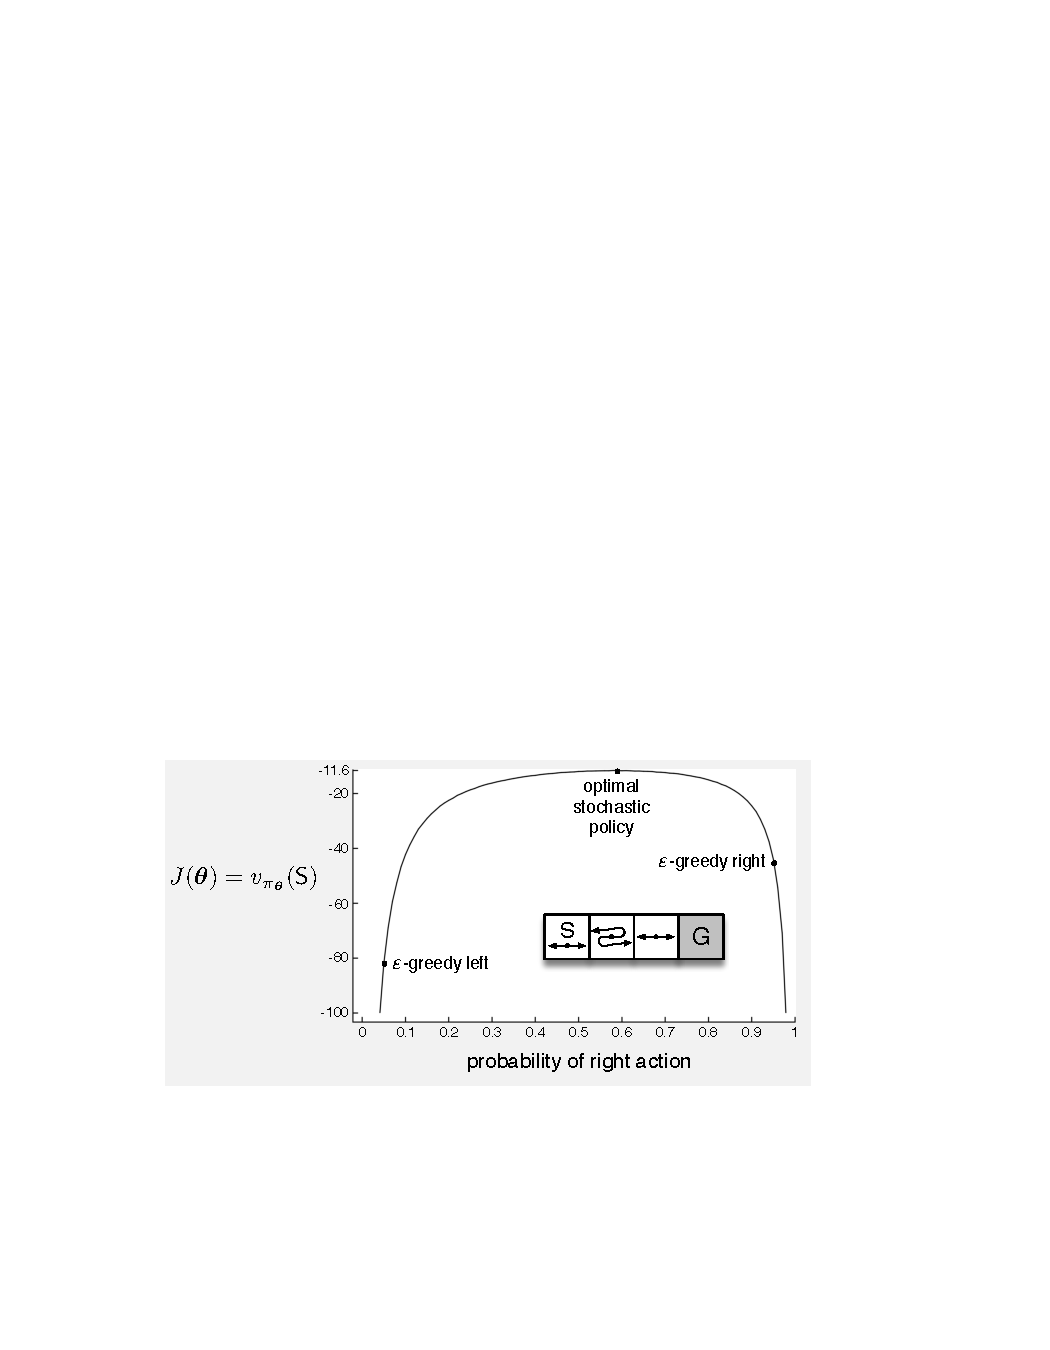
\includegraphics[height=0.5\textheight]{fig/lec11/Short_Corridor_Problem.pdf}
\caption{Short-corridor problem with $\varepsilon=0.1$ (source: R. Sutton and G. Barto, Reinforcement learning: an introduction, 2018, \href{https://creativecommons.org/licenses/by-nc-nd/2.0/}{CC BY-NC-ND 2.0})}
\label{fig:Short_Corridor_Problem}
\end{figure}
}

%%%%%%%%%%%%%%%%%%%%%%%%%%%%%%%%%%%%%%%%%%%%%%%%%%%%%%%%%%%%%
%% REINFORCE Comparison (2) %%
%%%%%%%%%%%%%%%%%%%%%%%%%%%%%%%%%%%%%%%%%%%%%%%%%%%%%%%%%%%%%
\frame{\frametitle{REINFORCE example: short-corridor problem (2)}
\begin{figure}
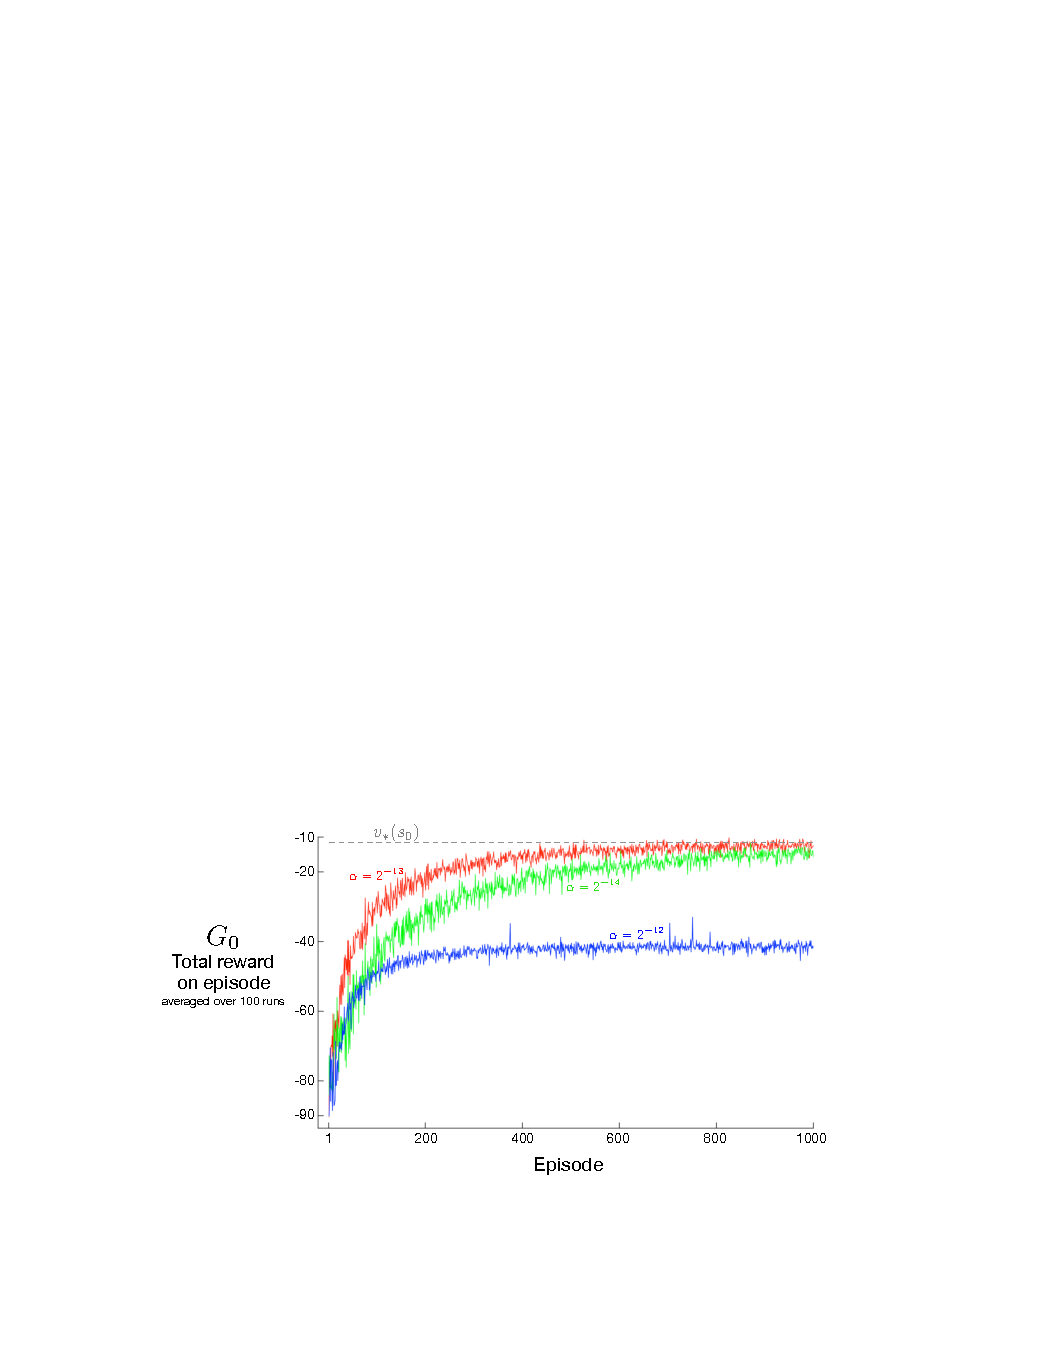
\includegraphics[height=0.65\textheight]{fig/lec11/REINFORCE_short_corridor.pdf}
\caption{Comparison of Monte Carlo policy gradient approach on short-corridor problem from \figref{fig:Short_Corridor_Problem} for different learning rates (source: R. Sutton and G. Barto, Reinforcement learning: an introduction, 2018, \href{https://creativecommons.org/licenses/by-nc-nd/2.0/}{CC BY-NC-ND 2.0})}
\label{fig:REINFORCE_short_corridor}
\end{figure}
}

%%%%%%%%%%%%%%%%%%%%%%%%%%%%%%%%%%%%%%%%%%%%%%%%%%%%%%%%%%%%%
%% Baseline %%
%%%%%%%%%%%%%%%%%%%%%%%%%%%%%%%%%%%%%%%%%%%%%%%%%%%%%%%%%%%%%
\frame{\frametitle{Baseline}
\begin{itemize}
	\item Motivation: add a comparison term to the policy gradient to reduce variance while not affecting its expectation.\pause
	\item Introduce the \hl{baseline $b(\bm{x})$}:
\end{itemize}
\begin{equation}
	\nabla_{\bm{\theta}} J(\bm{\theta}) = \El{\left(q_{\pi}(\bm{x},\bm{u})\hl{-b(\bm{x})}\right)\nabla_{\bm{\theta}}\ln \pi(\bm{u}|\bm{x},\bm{\theta})}{\pi}.
\end{equation}\pause
\vspace{-0.3cm}
\begin{itemize}
	\item Since $b(\bm{x})$ is only depending on the state but not on the actions/policy we did not change the policy gradient in expectation:
\end{itemize}
\vspace{0.3cm}
\begin{equation*}
	\nabla_{\bm{\theta}} J(\bm{\theta}) = \El{q_{\pi}(\bm{x},\bm{u})\nabla_{\bm{\theta}}\ln \pi(\bm{u}|\bm{x},\bm{\theta})}{\pi}- \underbrace{\El{b(\bm{x})\nabla_{\bm{\theta}}\ln \pi(\bm{u}|\bm{x},\bm{\theta})}{\pi}}_{=0}.
\end{equation*}\pause
\begin{itemize}
	\item Consequently, the Monte Carlo policy parameter update yields:
\end{itemize}
		\begin{equation*}
			\bm{\theta}_{k+1} = \bm{\theta}_k + \alpha\gamma^k \left(g_k-b(\bm{x}_k)\right) \nabla_{\bm{\theta}}\ln \pi(\bm{u}_k|\bm{x}_k,\bm{\theta}_k).
		\end{equation*}
}

%%%%%%%%%%%%%%%%%%%%%%%%%%%%%%%%%%%%%%%%%%%%%%%%%%%%%%%%%%%%%
%% Advantage %%
%%%%%%%%%%%%%%%%%%%%%%%%%%%%%%%%%%%%%%%%%%%%%%%%%%%%%%%%%%%%%
\frame{\frametitle{Advantage function}
\begin{itemize}
	\item Intuitive choice of the baseline is the state value $b(\bm{x})=v_{\pi}(\bm{x})$.
	\item The resulting policy gradient becomes
	\begin{equation}
	\nabla_{\bm{\theta}} J(\bm{\theta}) = \El{\left(q_{\pi}(\bm{x},\bm{u})-v_{\pi}(\bm{x})\right)\nabla_{\bm{\theta}}\ln \pi(\bm{u}|\bm{x},\bm{\theta})}{\pi}.
\end{equation}\pause
\item Here, the difference between action and state value is the \hl{advantage function}
	\begin{equation}
	a_\pi(\bm{x},\bm{u})= q_{\pi}(\bm{x},\bm{u})-v_{\pi}(\bm{x}) .
\end{equation}\pause
\item Interpretation: value difference taking (arbitrary) action $\bm{u}$ and thereafter following policy $\pi$ compared to the state value following same policy (i.e., choosing $\bm{u}\sim\pi$) given the state.\pause
\item Hence, we might rewrite to:
	\begin{equation}
	\nabla_{\bm{\theta}} J(\bm{\theta}) = \El{a_\pi(\bm{x},\bm{u})\nabla_{\bm{\theta}}\ln \pi(\bm{u}|\bm{x},\bm{\theta})}{\pi}.
\end{equation}
\end{itemize}
}

%%%%%%%%%%%%%%%%%%%%%%%%%%%%%%%%%%%%%%%%%%%%%%%%%%%%%%%%%%%%%
%% Algorithmic Implementation: Monte Carlo Policy Gradient with Baseline%%
%%%%%%%%%%%%%%%%%%%%%%%%%%%%%%%%%%%%%%%%%%%%%%%%%%%%%%%%%%%%%
\frame{\frametitle{Algo. implementation: MC policy gradient with baseline}
\vspace{-0.1cm}
\begin{itemize}
	\item Implementation requires approximation $b(\bm{x})\approx \hat{v}(\bm{x},\bm{w})$.
	\item Hence, we are learning two parameter sets $\bm{\theta}$ and $\bm{w}$. 
	\item Keep using sampled return as action-value estimate: $q_{\pi}(\bm{x},\bm{u}) \approx g_k$.
\end{itemize}
\setlength{\algomargin}{0.5em}
\begin{algorithm}[H]
\SetKwInput{Input}{input} 
\SetKwInput{Output}{output}
\SetKwInput{Init}{init}
\SetKwInput{Param}{parameter}
\Input{a differentiable policy function $\pi(\bm{u}|\bm{x},\bm{\theta})$ and state-value function $\hat{v}(\bm{x},\bm{w})$}
\Param{step sizes $\{\alpha_{w}, \alpha_{\theta}\}\in\left\{\mathbb{R}|0<\alpha<1\right\}$}
\Init{parameter vectors $\bm{w}\in\mathbb{R}^{\zeta}$ and $\bm{\theta}\in\mathbb{R}^d$ arbitrarily}
 \For{$j=1,2,\ldots,$ episodes}{
		generate an episode following $\pi(\cdot|\cdot,\bm{\theta})$: $\bm{x}_{0}, \bm{u}_{0}, r_{1},\ldots,\bm{x}_{T}$ \;  
		\For{$k=0,1,\ldots, T-1$ time steps}{
			$g\leftarrow \sum_{i=k+1}^T\gamma^{i-k-1}r_i$\;
			$\delta \leftarrow g - \hat{v}(\bm{x}_k, \bm{w})$\;
			$\bm{w} \leftarrow \bm{w}+\alpha_w\delta\nabla_{\bm{w}}\hat{v}(\bm{x}_k,\bm{w})$\;
			$\bm{\theta} \leftarrow \bm{\theta} + \alpha_{\theta} \gamma^k \delta \nabla_{\bm{\theta}}\ln \pi(\bm{u}_k|\bm{x}_k,\bm{\theta})$\; 
		}
	}
\caption{Monte Carlo policy gradient with baseline (output: parameter vector $\bm{\theta}^*$ for $\pi^*(\bm{u}|\bm{x},\bm{\theta}^*)$) and $\bm{w}^*$ for $\hat{v}^*(\bm{x}, \bm{w}^*))$}
\label{algo:MC_policy_gradient_baseline}
\end{algorithm}
}

%%%%%%%%%%%%%%%%%%%%%%%%%%%%%%%%%%%%%%%%%%%%%%%%%%%%%%%%%%%%%
%% REINFORCE Comparison %%
%%%%%%%%%%%%%%%%%%%%%%%%%%%%%%%%%%%%%%%%%%%%%%%%%%%%%%%%%%%%%
\frame{\frametitle{REINFORCE comparison w/o baseline}
\begin{figure}
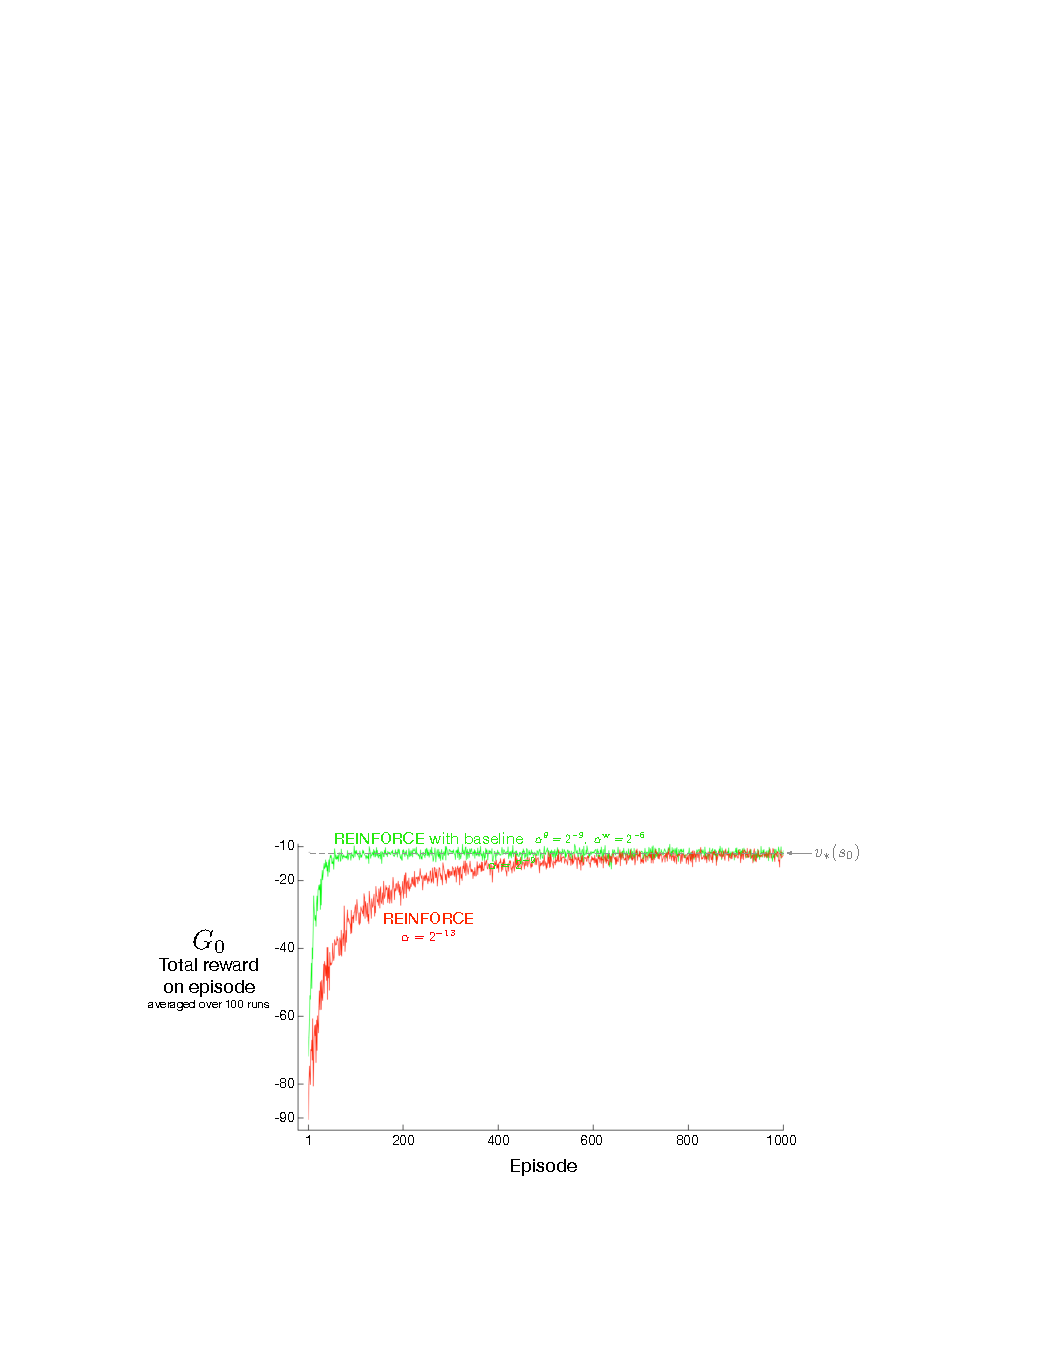
\includegraphics[height=0.65\textheight]{fig/lec11/REINFORCE_short_corridor_baseline.pdf}
\caption{Comparison of Monte Carlo policy gradient on short-corridor problem from \figref{fig:Short_Corridor_Problem} where both algorithms' learning rates have been tuned (source: R. Sutton and G. Barto, Reinforcement learning: an introduction, 2018, \href{https://creativecommons.org/licenses/by-nc-nd/2.0/}{CC BY-NC-ND 2.0})}
\label{fig:REINFORCE_short_corridor_baseline}
\end{figure}
}

%%%%%%%%%%%%%%%%%%%%%%%%%%%%%%%%%%%%%%%%%%%%%%%%%%%%%%%%%%%%%%%%%%
\section{Actor-critic methods} 
%%%%%%%%%%%%%%%%%%%%%%%%%%%%%%%%%%%%%%%%%%%%%%%%%%%%%%%%%%%%%%%%%%
\begin{frame}
\frametitle{Table of contents}
\tableofcontents[currentsection]
\end{frame}

%%%%%%%%%%%%%%%%%%%%%%%%%%%%%%%%%%%%%%%%%%%%%%%%%%%%%%%%%%%%%
%% General Actor-Critic Idea %%
%%%%%%%%%%%%%%%%%%%%%%%%%%%%%%%%%%%%%%%%%%%%%%%%%%%%%%%%%%%%%
\frame{\frametitle{General actor-critic idea}
Conclusion of Monte Carlo policy gradient with baseline:
\begin{itemize}
	\item Will learn an unbiased policy gradient.
	\item As the other MC-based methods: learns slowly due to high variance.
	\item Updates only available after full episodes.
\end{itemize}\pause
\vspace{0.5cm}
Alternative: use an additional function approximator, the so-called \hl{critic}, to estimate $q_{\pi}$ (i.e., approximate policy gradient):
\begin{equation*}
\begin{split}
	 v(\bm{x})&\approx \hat{v}(\bm{x}, \bm{w}_v),\\
	q(\bm{x},\bm{u})&\approx \hat{q}(\bm{x}, \bm{u}, \bm{w}_q),\\
	a(\bm{x},\bm{u})&\approx \hat{q}(\bm{x}, \bm{u}, \bm{w}_q) - \hat{v}(\bm{x}, \bm{w}_v). 
\end{split}	
\end{equation*}\pause
\begin{itemize}
  \item Realization: any prediction tool discussed so far (TD(0), LSTD,...).\pause
	\item Potential: we can use online step-by-step updates to estimate $\hat{q}$.\pause
	\item Disadvantage: we would train two value estimates by $\bm{w}_v$ and $\bm{w}_q$. 
\end{itemize}
}

%%%%%%%%%%%%%%%%%%%%%%%%%%%%%%%%%%%%%%%%%%%%%%%%%%%%%%%%%%%%%
%% Integrating the Advantage Function %%
%%%%%%%%%%%%%%%%%%%%%%%%%%%%%%%%%%%%%%%%%%%%%%%%%%%%%%%%%%%%%
\frame{\frametitle{Integrating the advantage function}
\begin{itemize}
	\item The TD error is 
\begin{equation}
	\delta_\pi = r + \gamma v_\pi(\bm{x}') - v_\pi(\bm{x}). \pause\vspace{-0.3cm}
\end{equation}
\item In expectation the TD error is equivalent to the advantage function
\begin{equation}
\begin{split}
	\El{\delta_\pi|\bm{x}, \bm{u}}{\pi} &= \El{r + \gamma v_\pi(\bm{x}')|\bm{x}, \bm{u}}{\pi} - v_\pi(\bm{x})\\ 
																			&= q_\pi(\bm{x},\bm{u})- v_\pi(\bm{x})\\
																			&= a_\pi(\bm{x},\bm{u}) .
\end{split}
\end{equation}\pause
\item Hence, the TD error can be used to calculate the policy gradient:
	\begin{equation}
	\nabla_{\bm{\theta}} J(\bm{\theta}) = \El{\delta_\pi \nabla_{\bm{\theta}}\ln \pi(\bm{u}|\bm{x},\bm{\theta})}{\pi}.
\end{equation} \pause\vspace{-0.3cm}
\item This results in requiring only one function parameter set:
	\begin{equation}
	\delta_\pi \approx r + \gamma \hat{v}_\pi(\bm{x}', \bm{w}) - \hat{v}_\pi(\bm{x}, \bm{w}).
\end{equation} 
\end{itemize}
}

%%%%%%%%%%%%%%%%%%%%%%%%%%%%%%%%%%%%%%%%%%%%%%%%%%%%%%%%%%%%%
%% Actor-Critic Structure %%
%%%%%%%%%%%%%%%%%%%%%%%%%%%%%%%%%%%%%%%%%%%%%%%%%%%%%%%%%%%%%
\frame{\frametitle{Actor-critic structure}
\begin{itemize}
	\item Critic (policy evaluation) and actor (policy improvement) can be considered another form of generalized policy iteration (GPI).
	\item Online and on-policy algorithm for discrete and continuous action spaces with built-in exploration by stochastic policy functions.
\end{itemize}
\begin{figure}
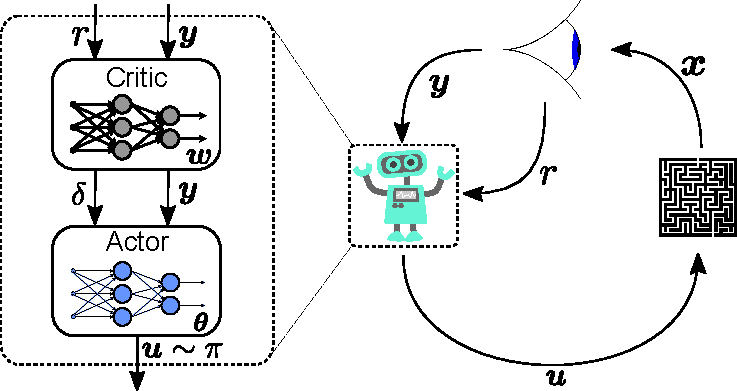
\includegraphics[height=0.5\textheight]{fig/lec11/Actor-Critic.pdf}
\caption{Simplified flow diagram of actor-critic-based RL}
\label{fig:Actor-Critic}
\end{figure}
}

%%%%%%%%%%%%%%%%%%%%%%%%%%%%%%%%%%%%%%%%%%%%%%%%%%%%%%%%%%%%%
%% Algorithmic Implementation:Actor-Critic with TD(0) Targets %%
%%%%%%%%%%%%%%%%%%%%%%%%%%%%%%%%%%%%%%%%%%%%%%%%%%%%%%%%%%%%%
\frame{\frametitle{Algo. implementation: actor-critic with TD(0) targets}
\begin{itemize}
	\item Analog to MC-based policy gradient optional discounting on the gradient updates is introduced.
\end{itemize}
\setlength{\algomargin}{0.5em}
\begin{algorithm}[H]
\SetKwInput{Input}{input} 
\SetKwInput{Output}{output}
\SetKwInput{Init}{init}
\SetKwInput{Param}{parameter}
\Input{a differentiable policy function $\pi(\bm{u}|\bm{x},\bm{\theta})$ and state-value function $\hat{v}(\bm{x},\bm{w})$}
\Param{step sizes $\{\alpha_{w}, \alpha_{\theta}\}\in\left\{\mathbb{R}|0<\alpha<1\right\}$}
\Init{parameter vectors $\bm{w}\in\mathbb{R}^{\zeta}$ and $\bm{\theta}\in\mathbb{R}^d$ arbitrarily}
 \For{$j=1,2,\ldots,$ episodes}{
		initialize $\bm{x}_0$\; 
		\For{$k=0,1,\ldots, T-1$ time steps}{
			apply $\bm{u}_k \sim \pi(\cdot|\bm{x}_k, \bm{\theta})$ and observe $\bm{x}_{k+1}$ and $r_{k+1}$\;
			$\delta \leftarrow r_{k+1} + \gamma \hat{v}(\bm{x}_{k+1}, \bm{w})- \hat{v}(\bm{x}_k, \bm{w})$\;
			$\bm{w} \leftarrow \bm{w}+\alpha_w\delta\nabla_{\bm{w}}\hat{v}(\bm{x}_k,\bm{w})$\;
			$\bm{\theta} \leftarrow \bm{\theta} + \alpha_{\theta} \gamma^k \delta \nabla_{\bm{\theta}}\ln \pi(\bm{u}_k|\bm{x}_k,\bm{\theta})$\; 
		}
	}
\caption{Actor-critic for episodic tasks using TD(0) targets (output: parameter vector $\bm{\theta}^*$ for $\pi^*(\bm{u}|\bm{x},\bm{\theta}^*)$) and $\bm{w}^*$ for $\hat{v}^*(\bm{x}, \bm{w}^*))$}
\label{algo:actor_critic_TD0}
\end{algorithm}
}



%%%%%%%%%%%%%%%%%%%%%%%%%%%%%%%%%%%%%%%%%%%%%%%%%%%%%%%%%%%%%
%% Actor-Critic Generalization %%
%%%%%%%%%%%%%%%%%%%%%%%%%%%%%%%%%%%%%%%%%%%%%%%%%%%%%%%%%%%%%
\frame{\frametitle{Actor-critic generalization}
\begin{itemize}
	\item Using the TD(0) error as the target to train the critic is convenient. \pause
	\item However, the usual alternatives can be applied to train $\hat{v}(\bm{x}, \bm{w})$.\pause
	\item $n$-step bootstrapping: 
	\begin{equation*}
		 v(\bm{x}_k) \approx r_{k+1}+\gamma r_{k+2}+\cdots+\gamma^{n-1} r_{k+n}+\gamma^{n} \hat{v}_{k+n-1}(\bm{x}_{k+n}, \bm{w}).
	\end{equation*}\pause\vspace{-0.3cm}
	\item $\lambda$-return (forward view): 
	\begin{equation*}
		 v(\bm{x}_k) \approx(1-\lambda)\sum_{n=1}^{T-k-1}\lambda^{(n-1)}g_{k:k+n} + \lambda^{T-k-1}g_k.
	\end{equation*}\pause\vspace{-0.3cm}
	\item TD($\lambda$) using eligibility traces (backward view):
		\begin{equation*}
			\begin{split}
				\bm{z}_k &=\gamma\lambda\bm{z}_{k-1}+\nabla_{\bm{w}}\hat{v}(\bm{x}_k,\bm{w}_k),\\
				\delta_k &=r_{k+1} + \gamma \hat{v}(\bm{x}_{k+1}, \bm{w}_k) -\hat{v}(\bm{x}_{k}, \bm{w}_k).
			\end{split}	
		\end{equation*}
\end{itemize}
}

%%%%%%%%%%%%%%%%%%%%%%%%%%%%%%%%%%%%%%%%%%%%%%%%%%%%%%%%%%%%%
%% Algorithmic Implementation:Actor-Critic with TD($\lambda$) Targets %%
%%%%%%%%%%%%%%%%%%%%%%%%%%%%%%%%%%%%%%%%%%%%%%%%%%%%%%%%%%%%%
\frame{\frametitle{Algo. implementation: actor-critic with TD($\lambda$) targets}
\setlength{\algomargin}{0.5em}
\begin{algorithm}[H]
\SetKwInput{Input}{input} 
\SetKwInput{Output}{output}
\SetKwInput{Init}{init}
\SetKwInput{Param}{parameter}
\Input{a differentiable policy function $\pi(\bm{u}|\bm{x},\bm{\theta})$}
\Input{a differentiable state-value function $\hat{v}(\bm{x},\bm{w})$}
\Param{$\{\alpha_{w}, \alpha_{\theta}\}\in\left\{\mathbb{R}|0<\alpha<1\right\}$, $\{\lambda_{w}, \lambda_{\theta}\}\in\left\{\mathbb{R}|0 \leq \lambda \leq 1\right\}$}
\Init{parameter vectors $\bm{w}\in\mathbb{R}^{\zeta}$ and $\bm{\theta}\in\mathbb{R}^d$ arbitrarily}
 \For{$j=1,2,\ldots,$ episodes}{
		initialize $\bm{x}_0$, $\bm{z}_w=0$, $\bm{z}_{\theta}=0$\; 
		\For{$k=0,1,\ldots, T-1$ time steps}{
			apply $\bm{u}_k \sim \pi(\cdot|\bm{x}_k, \bm{\theta})$ and observe $\bm{x}_{k+1}$ and $r_{k+1}$\;
			$\delta \leftarrow r_{k+1} + \gamma \hat{v}(\bm{x}_{k+1}, \bm{w})- \hat{v}(\bm{x}_k, \bm{w})$\;
			$\bm{z}_w \leftarrow \gamma\lambda_w\bm{z}_w + \nabla_{\bm{w}}\hat{v}(\bm{x}_k,\bm{w})$\;
			$\bm{z}_{\theta} \leftarrow \gamma\lambda_d\bm{z}_{\theta} + \gamma^k \nabla_{\bm{\theta}}\ln \pi(\bm{u}_k|\bm{x}_k,\bm{\theta})$\;
			$\bm{w} \leftarrow \bm{w}+\alpha_w\delta\bm{z}_w$\;
			$\bm{\theta} \leftarrow \bm{\theta} + \alpha_{\theta} \delta \bm{z}_{\theta}$\; 
		}
	}
\caption{Actor-critic for episodic tasks using TD($\lambda$) targets (output: parameter vector $\bm{\theta}^*$ for $\pi^*(\bm{u}|\bm{x},\bm{\theta}^*)$) and $\bm{w}^*$ for $\hat{v}^*(\bm{x}, \bm{w}^*))$}
\label{algo:actor_critic_TD_lambda}
\end{algorithm}
}

%%%%%%%%%%%%%%%%%%%%%%%%%%%%%%%%%%%%%%%%%%%%%%%%%%%%%%%%%%%%%
%% Summary %%
%%%%%%%%%%%%%%%%%%%%%%%%%%%%%%%%%%%%%%%%%%%%%%%%%%%%%%%%%%%%%
\begin{frame}
\frametitle{Summary: what you've learned today}
\begin{itemize}
	\item Policy-based methods are a new class within the RL toolbox.
	\begin{itemize}
		\item Instead of learning a policy indirectly from a value the policy is directly parametrized.\pause
		\item The policy function allows discrete and continuous actions with inherent stochastic exploration.\pause
	\end{itemize}
	\item Solving the underlying optimization task is complex. However, the policy gradient theorem provides a suitable theoretical baseline for gradient-based optimization.\pause
	\item Anyhow, to calculate policy gradients we require a value estimate.
	\begin{itemize}
		\item Monte Carlo prediction is straightforward, but comes with high variance and slow learning.\pause
		\item Adding a state-dependent baseline comparison does not change the policy gradient in expectation but enables decreasing the variance.\pause
	\end{itemize}
	\item Extending this idea naturally leads to integrating a critic network, i.e., an additional function approximation to estimate the value.\pause
	\item The critic can be fed by the usual targets (TD(0), TD($\lambda$),...).
\end{itemize}
\end{frame}